%% Type de document et encodage de la police
\documentclass[a4paper]{article}
\usepackage[utf8x]{inputenc}
\usepackage[T1]{fontenc}
\usepackage[colorlinks=true, allcolors=black]{hyperref}
% \usepackage[french]{babel}

%% Initialise la taille des pages et des marges
\usepackage[a4paper, top=3cm, bottom=3cm, left=2cm, right=2cm, marginparwidth=2cm]{geometry}

%% Packs utiles
\usepackage{amsmath}
\usepackage{graphicx}

%% Commandes perso
\renewcommand{\arraystretch}{1.2} %% row 20% longer
\renewcommand{\contentsname}{Table des matières}

%% Pour les exemples
\usepackage{mdframed}
\newmdenv[topline=false, bottomline=false, rightline=false, skipabove=\topsep, skipbelow=\topsep]{example}

%% Pour les diagrammes
\usepackage{tikz}
\tikzstyle{incolore} = [rectangle, rounded corners, draw=black, minimum height=1cm, minimum width=3cm, text width=3cm, text centered]


\title{Pfsense - OpenVPN \& Captive Portal}
\author{Grégoire Roumache}
\date{Mars 2021}

\begin{document}

\maketitle















\section{Installations \& Configurations}










\subsection{Configuration internet explorer - windows server}





Pour pouvoir configurer pfsense àpd internet explorer, il faut:
\begin{enumerate}
    \item ouvrir le \textit{server manager}
    \item dans le menu de gauche, cliquer sur \textit{local server}
    \item au centre à droite, cliquer sur \textit{On} à droite de \textit{IE Enhanced Security Configuration}
    \item désactiver la sécurité (cliquer sur \textit{off} pour les 2 paramètres), puis cliquer sur \textit{ok}
\end{enumerate}
\textbf{Remarque}: si internet explorer était ouvert, il faut le fermer puis le rouvrir pour que le changement ait lieu.










\subsection{Installation active directory - windows server}





\textcolor{red}{\textbf{Attention !}} Il faut configurer la machine windows serveur en ip statique, avec le DNS = 127.0.0.1.
\begin{enumerate}
    \item ouvrir le \textit{server manager}
    \item en haut à droite, cliquer sur \textit{manage}, puis sur \textit{add roles and features}
    \item à gauche dans \textit{server roles}, sélectionner \textit{active directory domain services}
    \item cliquer sur \textit{add features} dans la popup, puis continuer jusqu'à l'installation
    \item quand un signe danger apparaît en haut à droite, cliquer dessus
    \item cliquer sur \textit{promote this server to a domain controller}
    \item sélectionner l'option \textit{add a new forest}, et ajouter le nom de domaine (ex: \textit{domaine.local})
    \item ensuite, ajouter le mot de passe DSRM: \textit{Tigrou007}, et terminer la configuration
\end{enumerate}










\subsection{Créer un groupe d'utilisateurs sur active directory - windows server}





\begin{itemize}
    \item Ajouter un groupe d'utilisateurs:
    \begin{enumerate}
        \item dans le \textit{server manager}, cliquer sur \textit{tools} en haut à droite
        \item ouvrir \textit{active directory users and computers}
        \item faire un clic-droit sur \textit{<domaine>/users}, puis cliquer sur \textit{new}, puis sur \textit{group}
        \item compléter le formulaire 
    \end{enumerate}
    \item Ajouter des utilisateurs à un groupe:
    \begin{enumerate}
        \item dans le \textit{server manager}, cliquer sur \textit{tools} en haut à droite
        \item ouvrir \textit{active directory users and computers}
        \item faire un clic-droit sur \textit{<domaine>/users}, puis cliquer sur \textit{new}, puis sur \textit{group}
    \end{enumerate}
    \item Ajouter des utilisateurs:
    \begin{enumerate}
        \item dans le \textit{server manager}, cliquer sur \textit{tools} en haut à droite
        \item ouvrir \textit{active directory users and computers}
        \item cliquer sur \textit{<domaine>/users}, faire un clic-droit sur le groupe, puis cliquer sur \textit{properties}
        \item dans l'onglet \textit{members}, cliquer sur \textit{add}
        \item écrire les noms des utilisateurs à ajouter, cliquer sur \textit{check names}, puis \textit{ok}
    \end{enumerate}
\end{itemize}










\subsection{Installer et configurer RADIUS - windows server}





\textcolor{red}{\textbf{Attention !}} Il faut que le parefeu soit désactivé pour que ça fonctionne correctement.
\begin{itemize}
    \item Installer RADIUS:
    \begin{enumerate}
        \item ouvrir le \textit{server manager}
        \item en haut à droite, cliquer sur \textit{manage}, puis sur \textit{add roles and features}
        \item à gauche dans \textit{server roles}, sélectionner \textit{network policy and access services}
        \item cliquer sur \textit{add features} dans la popup, puis continuer jusqu'à l'installation
        \item continuer et installer le service
    \end{enumerate}
    \item Configurer RADIUS:
    \begin{enumerate}
        \item dans le \textit{server manager}, cliquer sur \textit{tools} en haut à droite
        \item ouvrir \textit{network policy server}
        \item dans le menu de gauche, faire un clic gauche sur \textit{radius clients and servers/radius clients}
        \item cliquer sur \textit{new}, et compléter le formulaire:
        \begin{itemize}
            \item Friendly name = VPN pfsense (pas d'impact sur le fonctionnement)
            \item Address (IP or DNS) = IP du parefeu pfsense
            \item Shared secret template = None
            \item Manual/Generate = Generate
            \item Shared secret $\implies$ cliquer sur \textit{generate}
        \end{itemize}
        \textbf{Remarque}: copier le secret partagé dans un fichier texte, pour l'ajouter au parefeu plus tard.
        \item cliquer sur \textit{ok}
        \item dans le menu de gauche, faire un clic gauche sur \textit{policies/network policies}
        \item cliquer sur \textit{new}, et ajouter un nom (ex: \textit{allow pfsense}), puis cliquer sur \textit{next}
        \item cliquer sur \textit{add}, sélectionner \textit{windows groups}, puis cliquer sur \textit{add}
        \item cliquer sur \textit{add groups}, taper le nom du groupe (ex: \textit{VPNusers})
        \item cliquer sur \textit{check names}, puis sur \textit{ok}, encore sur \textit{ok}, puis sur \textit{next}
        \item sélectionner \textit{access granted}, puis cliquer sur \textit{next}
        \item dans \textit{configure authentification method}, sélectionner uniquement \textit{MS-CHAP-v2}
        \item cliquer 3 fois sur \textit{next}, puis sur \textit{finish}
    \end{enumerate}
\end{itemize}
\textbf{Remarque}: il faut que la stratégie créée ait un \textit{processing order} plus petit que les autres pour que le trafic ne soit pas bloqué.
\begin{center} 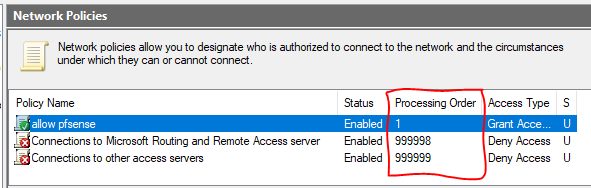
\includegraphics[width=0.65\linewidth]{images/network-policies-order-01.PNG} \end{center}










\subsection{Configuration routeur - routeur debian}





Pour transformer la machine debian en routeur, il faut décommenter la ligne suivante dans \texttt{/etc/sysctl.conf}:
\begin{example} \begin{verbatim}
net.ipv4.ip_forward=1
\end{verbatim} \end{example}
Remarque: il faut ajouter des default gateways/routes statiques sur toutes les machines.










\subsection{Configuration de base - pfsense}





\begin{center} 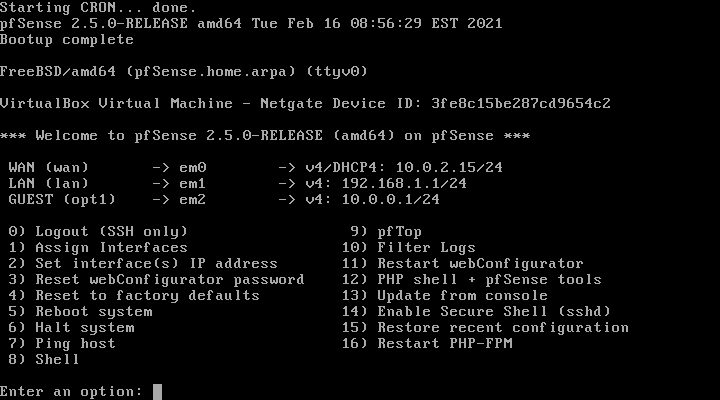
\includegraphics[width=0.85\linewidth]{images/pfsense-01.PNG} \end{center}
Il faut configurer pour avoir comme sur l'image, pour cela:
\begin{enumerate}
    \item aller dans l'option 1 - mettre les interfaces dans le réseau auquelles elles appartiennent (wan, lan, guest/opt1)
    \item ne pas créer de vlans
    \item aller dans l'option 2 - mettre em0 en dhcp, le reste en statique
    \item désactiver l'ipv6
    \item mettre non à "do you want to revert to http as the webconfigurator protocol?"
\end{enumerate}










\subsection{Configuration parefeu nat - pfsense}





\begin{enumerate}
    \item ouvrir l'interface web de pfsense
    \item aller sur \textit{firewall/nat/outbound}
    \item sélectionner le mode \textit{automatic oubound nat rule generation} et enregistrer
\end{enumerate}










\subsection{Configuration parefeu règles - pfsense}





\begin{enumerate}
    \item ouvrir l'interface web de pfsense
    \item aller sur \textit{firewall/rules/guest} ou sur \textit{firewall/rules/wan}
    \item cliquer sur \textit{add} pour ajouter une nouvelle règle
    \item modifier les protocoles et les sources/destinations autorisées
    \item enregistrer et appliquer la nouvelle règle
\end{enumerate}
\textcolor{red}{\textbf{Attention!}}
\begin{itemize}
    \item Il faut que le firewall \textbf{et les routes} soient bien configurées pour que les manips fonctionnent.
    \item Si l'interface WAN est connectée à un réseau privé (10/8, 172.16/12, 192.168/16), il faut désactiver la règle qui bloque ce traffic.
\end{itemize}










\subsection{Configuration routes statiques - pfsense}





\textcolor{red}{\textbf{Attention!}} Il faut que le firewall \textbf{et les routes} soient bien configurées pour que les manips fonctionnent.
\begin{enumerate}
    \item ouvrir l'interface web de pfsense
    \item aller sur \textit{system/routing/static routes}
    \item cliquer sur \textit{add}, puis ajouter le réseau, le masque
    \item enregistrer et appliquer la nouvelle route
\end{enumerate}










\subsection{Certificats (CA, CR, import, export) - pfsense} \label{subsec:certificatsPfsense}





\begin{itemize}


\item Créer une CA (= certificate authority):
\begin{enumerate}
    \item ouvrir l'interface web de pfsense
    \item aller sur \textit{system/certificate manager/ca}
    \item rentrer un nom pour la CA (ex: \textit{server-ca})
    \item sélectionner la méthode \textit{create an internal certificate authority}
    \item enregistrer la CA
\end{enumerate}
\textbf{Remarque}: il ne peut y avoir qu'une CA pour toute l'infra - à moins de faire des CA intermédiaires mais on ne fait pas ça dans le cours.


\item Créer un certificat:
\begin{enumerate}
    \item ouvrir l'interface web de pfsense
    \item aller sur \textit{system/certificate manager/certificates}
    \item cliquer sur \textit{add}, puis sélectionner la méthode \textit{create an internal certificate}
    \item donner un nom au certificat, sélectionner la bonne CA
    \item dans \textit{common name}, donner le nom du site sur lequel le certificat va aller (ex: \textit{siteA})
    \item dans \textit{certificate type}, sélectionner \textit{user certificate}
    \item dans \textit{alternative names}, sélectionner \textit{fqdn or hostname} et ajouter le nom du site sur lequel le certificat va aller (ex: \textit{siteA})
\end{enumerate}


\item Exporter un certificat/une clé:
\begin{enumerate}
    \item ouvrir l'interface web de pfsense
    \item aller sur \textit{system/certificate manager/certificates}
    \item cliquer sur un de ces boutons:
    \begin{center}
        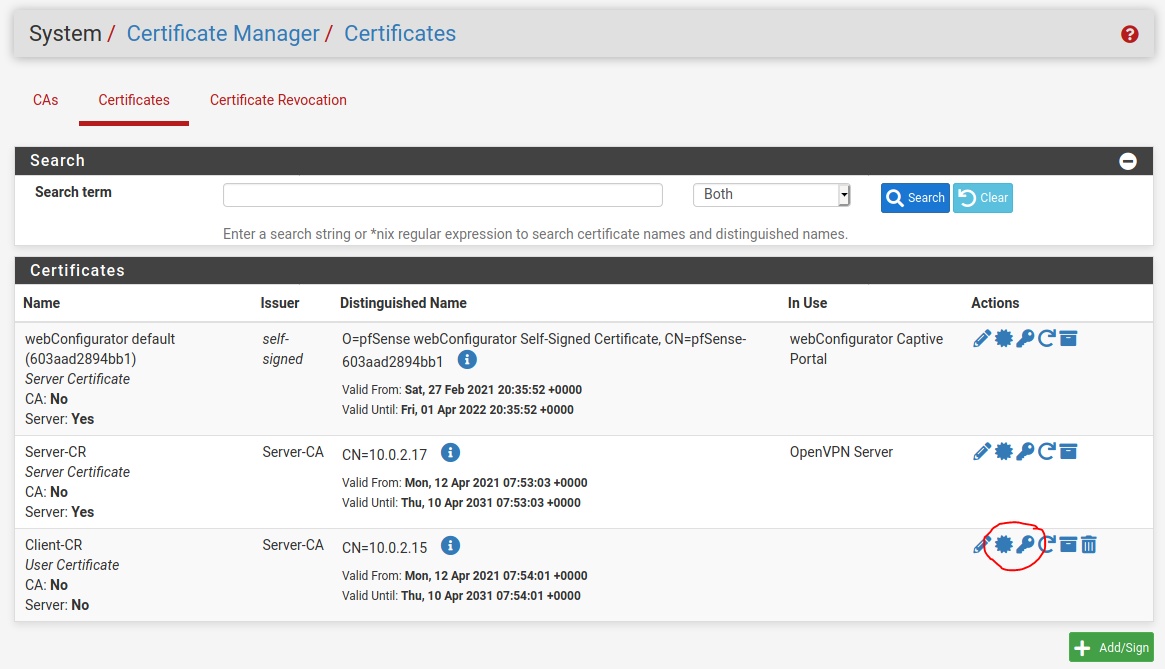
\includegraphics[width=0.99\linewidth]{images/CA-CR-export-01.PNG}
    \end{center}
\end{enumerate}
\textbf{Remarque}: il faut exporter le certificat de la CA et la clé + le certificat pour chaque client.


\item Importer un certificat:
\begin{enumerate}
    \item ouvrir l'interface web de pfsense
    \item aller sur \textit{system/certificate manager/certificates}
    \item cliquer sur \textit{add}, puis sélectionner la méthode \textit{import an existing certificate}
    \item donner un nom au certificat, puis copier les données du certificat et enregistrer le certificat
\end{enumerate}


\end{itemize}










\subsection{Ajouter RADIUS dans pfsense - pfsense}





\begin{enumerate}
    \item dans \texttt{system/user manager/authentification servers}, cliquer sur \textit{add}
    \begin{itemize}
        \item Descriptive name = RADIUS
        \item Type = RADIUS–Hostname or IP address = 192.168.1.2 (= adresse du serveur radius)
        \item Shared Secret = copier le secret généré pour ce parefeu sur le serveur radius
        \item Services offered = Authentication and Accounting
        \item Authentication port value = 1812
        \item Accounting port value = 1813
        \item RADIUS NAS IP Attribute = LAN - 192.168.1.1
    \end{itemize}
    \item cliquer sur \textit{save}
    \item dans \texttt{diagnostics/authentication}, tester la connexion d'un utilisateur à radius
\end{enumerate}










\subsection{Configuration FreeRadius - serveur debian}





...















\section{Labos}










\subsection{Captive Portal (accès internet sur un réseau invité)}





\begin{center} 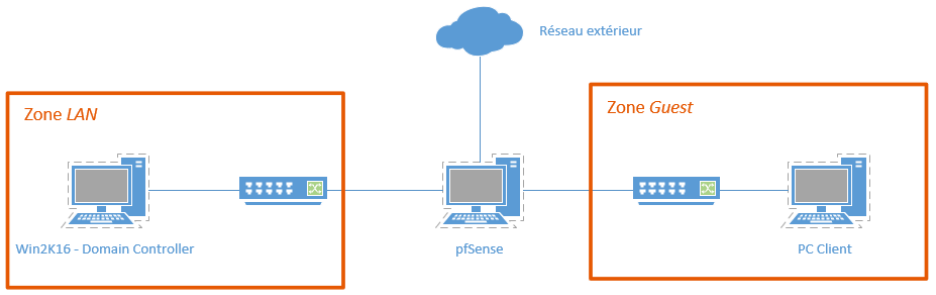
\includegraphics[width=0.99\linewidth]{images/captive-portal-01.PNG} \end{center}
\textcolor{red}{\textbf{Attention!}} Il faut que le firewall et les routes soient bien configurées.
\begin{itemize}

\item Activer le captive portal:
\begin{enumerate}
    \item aller sur \texttt{services/captive portal}, et cliquer sur \textit{add}
    \begin{itemize}
        \item Zone name = GUEST
        \item Zone description = Zone for guests
    \end{itemize}
    \item cliquer sur \textit{save \& continue}
    \item sur \texttt{services/captive portal/guest/configuration}
    \begin{itemize}
        \item Enable captive portal = cocher la case
        \item Interface = GUEST
        \item After authentication Redirection URL = \url{https://youtu.be/dQw4w9WgXcQ} (laisser vide)
        \item Authentification Method = Use an Authentification backend
        \item Authentification Server = Local Database
        \item Enable HTTPS login = cocher la case
        \item HTTPS server name = ip de la pfsense (interface guest)
    \end{itemize}
    \item cliquer sur \textit{save}
\end{enumerate}

\item Mettre l'interface guest en dhcp (si ce n'est pas déjà fait):
\begin{enumerate}
    \item aller sur \texttt{services/dhcp server/guest}
    \item cocher la case \textit{enable dhcp server on guest interface}
    \item cliquer sur \textit{save}
\end{enumerate}

\item Créer le groupe des utilisateurs qui peuvent se connecter à captive portal:
\begin{enumerate}
    \item aller sur \texttt{services/user manager/groups}, et cliquer sur \textit{add}
    \begin{itemize}
        \item Group Name = CaptivePortal
        \item Scope = Local
    \end{itemize}
    \item ajouter les membres si ils sont déjà créés (sinon, on peut les rajouter après)
    \item cliquer sur \textit{save}, puis éditer le groupe créé
    \item dans \textit{assigned privileges}, cliquer sur \textit{add}
    \item sélectionner le privilège \textit{user - services: captive portal login}, puis cliquer 2 fois sur \textit{save}
\end{enumerate}

\item Ajouter un utilisateur local:
\begin{enumerate}
    \item aller sur \texttt{services/user manager/users}, puis cliquer sur \textit{add}
    \item ajouter un \textit{username} et un mot de passe
    \item dans \textit{group membership}, cliquer sur \textit{captive portal}, puis sur \textit{move to "member of" list}
    \item cliquer sur \textit{save}
\end{enumerate}

\item Modifier le serveur d'authentication:
\begin{enumerate}
    \item aller sur \texttt{system/user manager/settings}
    \item dans \textit{authentification server}, sélectionner \textit{local database}
    \item cliquer sur \textit{save}
\end{enumerate}

\end{itemize}










\subsection{Captive Portal avec des vouchers (= codes d'accès wifi individuels)}





\begin{itemize}

\item Activer le captive portal:
\begin{enumerate}
    \item aller sur \texttt{services/captive portal}, et cliquer sur \textit{add}
    \begin{itemize}
        \item Zone name = GUEST
        \item Zone description = Zone for guests
    \end{itemize}
    \item cliquer sur \textit{save \& continue}
    \item sur \texttt{services/captive portal/guest/configuration}
    \begin{itemize}
        \item Enable captive portal = cocher la case
        \item Interface = GUEST
        \item After authentication Redirection URL = \url{https://youtu.be/dQw4w9WgXcQ} (laisser vide)
    \end{itemize}
    \item cliquer sur \textit{save}
    \item sur \texttt{services/captive portal/guest/vouchers}
    \item cocher la case \textit{enable the creation, generation and activations of rolls with vouchers}
    \item cliquer sur \textit{generate new keys}
    \item cliquer sur \textit{save}, puis cliquer sur \textit{add}
    \begin{itemize}
        \item Roll = 1 ($\implies$ numéro identifiant la génération de ces vouchers (pas important))
        \item Minutes per ticket = 1440
        \item Count = 150 ($\implies$ nombre de vouchers)
    \end{itemize}
    \item cliquer sur \textit{save}
\end{enumerate}

\item Modifier le serveur d'authentication:
\begin{enumerate}
    \item aller sur \texttt{system/user manager/settings}
    \item dans \textit{authentification server}, sélectionner \textit{local database}
    \item cliquer sur \textit{save}
\end{enumerate}

\end{itemize}










\subsection{Captive Portal avec RADIUS via active directory}





\begin{itemize}

\item Ajouter un serveur d'authentification:
\begin{enumerate}
    \item dans \texttt{system/user manager/authentification servers}, cliquer sur \textit{add}
    \begin{itemize}
        \item Descriptive name = RADIUS
        \item Type = RADIUS
        \item Hostname or IP address = 192.168.1.2 (= adresse du serveur radius)
        \item Shared Secret = copier le secret généré pour ce parefeu sur le serveur radius
        \item Services offered = Authentication and Accounting
        \item Authentication port value = 1812
        \item Accounting port value = 1813
        \item RADIUS NAS IP Attribute = LAN - 192.168.1.1
    \end{itemize}
    \item cliquer sur \textit{save}
\end{enumerate}

\item Tester l'authentification au serveur radius en allant sur \textit{diagnostics/authentification}.

\item Activer le captive portal:
\begin{enumerate}
    \item aller sur \texttt{services/captive portal}, et cliquer sur \textit{add}
    \begin{itemize}
        \item Zone name = GUEST
        \item Zone description = Zone for guests
    \end{itemize}
    \item cliquer sur \textit{save \& continue}
    \item sur \texttt{services/captive portal/guest/configuration}
    \begin{itemize}
        \item Enable captive portal = cocher la case
        \item Interface = GUEST
        \item After authentication Redirection URL = \url{https://youtu.be/dQw4w9WgXcQ} (laisser vide)
        \item Authentification Method = Use an Authentification backend
        \item Authentification Server = radius
        \item Enable HTTPS login = cocher la case
        \item HTTPS server name = ip de la pfsense (interface guest)
    \end{itemize}
    \item cliquer sur \textit{save}
\end{enumerate}

\item Modifier le serveur d'authentication:
\begin{enumerate}
    \item aller sur \texttt{system/user manager/settings}
    \item dans \textit{authentification server}, sélectionner \textit{radius}
    \item cliquer sur \textit{save}
\end{enumerate}

\end{itemize}










\subsection{Captive Portal - attaque man in the middle}





\begin{enumerate}
    \item désactiver le login en https sur le captive portal
    \item lancer le programme ettercap sur une kali dans le réseau guest
    \item une fois les ip du pc client et de pfsense trouvé, cliquer sur \textit{mitm} et lancer l'arp poisoning
    \item lancer wireshark et appliquer le filtre: \texttt{ip.src == <ip\_client> and ip.dst == <ip\_pfsense> and http}
    \item lancer une connexion sur un site en http (pour éviter la redirection https) et se connecter sur le captive portal
    \item obtenir les informations de connexion dans la requête http post dans wireshark
\end{enumerate}
\textbf{Remarque}: une fois qu'on a un compte de l'active directory, qu'est-ce qu'on peut en faire ?










\subsection{OpenVPN site to site avec clé partagée (pas dans le cours mais plus simple)}





\begin{center} 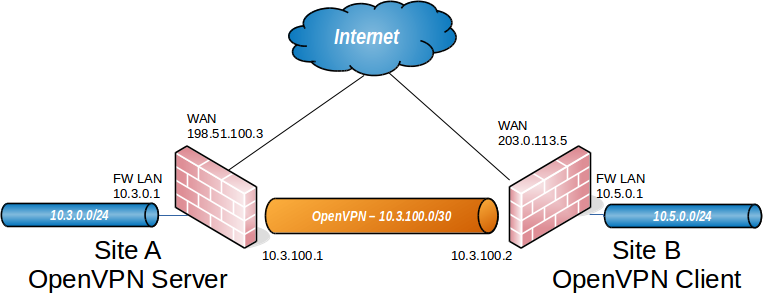
\includegraphics[width=0.99\linewidth]{images/openvpn-01.png} \end{center}

\begin{enumerate}
    \item sur l'openvpn serveur, dans \texttt{vpn/openvpn/servers}, ajouter une entrée:
    \begin{itemize}
        \item Server mode = Peer to Peer (Shared Key)
        \item IPv4 Tunnel Network = 10.0.3.0/24 (= réseau virtuel s2s)
        \item IPv4 Remote Network(s) = 192.168.2.0/24, 10.0.1.0/24 (= lans du côté openvpn client)
        \item éditer le serveur et exporter la clé \textit{shared key} sur l'openvpn client
    \end{itemize}
    \item sur l'openvpn client, dans \texttt{vpn/openvpn/clients}, ajouter une entrée:
    \begin{itemize}
        \item Server mode = Peer to Peer (Shared Key)
        \item Server host or address = 10.0.2.17 (= ip wan de l'openvpn serveur)
        \item Auto generate = décocher la case
        \item Shared Key = copier la clé exportée tantôt
        \item IPv4 Tunnel Network = 10.0.3.0/24 (= réseau virtuel s2s)
        \item IPv4 Remote Network(s) = 192.168.1.0/24, 10.0.0.0/24 (= lans du côté openvpn serveur)
    \end{itemize}
    \item sur l'openvpn client, dans \texttt{interfaces/interface assignments}, cliquer sur \textit{add}, puis sur \textit{save}
    \item sur l'openvpn client, dans \texttt{interfaces/<nouvelle\_interface>}:
    \begin{itemize}
        \item Enable interface = cocher la case
        \item Description = VPN-S2S
    \end{itemize}
    \item sur l'openvpn client, dans \texttt{status/openvpn}, redémarrer le service
    \item sur les 2 openvpn, dans \texttt{firewall/rules/wan}, ajouter une entrée:
    \begin{itemize}
        \item Protocol = UDP
        \item Port = 1194 (OpenVPN)
    \end{itemize}
    \item sur les 2 openvpn, dans \texttt{firewall/rules/wan}, désactiver la règle: \textit{block private networks}
    \item sur les 2 openvpn, dans \texttt{firewall/rules/OpenVPN}, ajouter une entrée:
    \begin{itemize}
        \item Protocol = any
    \end{itemize}
    \item sur l'openvpn client, dans \texttt{firewall/rules/VPN-S2S}, ajouter une entrée:
    \begin{itemize}
        \item Protocol = any
    \end{itemize}
\end{enumerate}










\subsection{OpenVPN site to site avec certificats}





\begin{enumerate}
    \item sur l'openvpn serveur, dans \texttt{system/certificate manager/cas}, ajouter une entrée:
    \begin{itemize}
        \item Descriptive Name = Server-CA
    \end{itemize}
    \item sur l'openvpn serveur, dans \texttt{system/certificate manager/certificates}, ajouter une entrée:
    \begin{itemize}
        \item Descriptive Name = Server-CR
        \item Common Name = 10.0.2.17 (= ip de l'openvpn serveur)
        \item Certificate Type = Server Certificate
    \end{itemize}
    \item sur l'openvpn serveur, dans \texttt{system/certificate manager/certificates}, ajouter une entrée:
    \begin{itemize}
        \item Descriptive Name = Client-CR
        \item Common Name = 10.0.2.15 (= ip de l'openvpn client)
    \end{itemize}
    \item importer le certificat de \textit{server-ca} et la clé et le certificat de \textit{client-cr} sur l'openvpn client
    \item sur l'openvpn serveur, dans \texttt{vpn/openvpn/servers}, ajouter une entrée:
    \begin{itemize}
        \item Use a TLS Key = décocher la case
        \item Server Certificate = Server-CR
        \item IPv4 Tunnel Network = 10.0.3.0/24 (= réseau virtuel s2s)
        \item IPv4 Local Network(s) = 10.0.0.0/24, 192.168.1.0/24 (= lans du côté openvpn serveur)
        \item IPv4 Remote network(s) = 10.0.1.0/24, 192.168.2.0/24 (= lans du côté openvpn client)
    \end{itemize}
    \item sur l'openvpn client, dans \texttt{vpn/openvpn/servers}, ajouter une entrée:
    \begin{itemize}
        \item Server host or address = 10.0.2.17 (= adresse wan de l'openvpn serveur)
        \item Server Port = faire correspondre ce port à celui utilisé sur le serveur (a priori 1194)
        \item Use a TLS Key = décocher la case
        \item Client Certificate = Client-CR
        \item IPv4 Tunnel Network = 10.0.3.0/24 (= réseau virtuel s2s)
        \item IPv4 Remote network(s) = 192.168.1.0/24, 10.0.0.0/24 (= lans du côté openvpn serveur)
    \end{itemize}
    \item sur l'openvpn client, dans \texttt{interfaces/interface assignments}, cliquer sur \textit{add}, puis sur \textit{save}
    \item sur l'openvpn client, dans \texttt{interfaces/<nouvelle\_interface>}:
    \begin{itemize}
        \item Enable interface = cocher la case
        \item Description = VPN-S2S
    \end{itemize}
    \item sur l'openvpn client, dans \texttt{status/openvpn}, redémarrer le service
    \item sur les 2 openvpn, dans \texttt{firewall/rules/wan}, ajouter une entrée:
    \begin{itemize}
        \item Protocol = UDP
        \item Port = 1194 (OpenVPN)
    \end{itemize}
    \item sur les 2 openvpn, dans \texttt{firewall/rules/wan}, désactiver la règle: \textit{block private networks}
    \item sur les 2 openvpn, dans \texttt{firewall/rules/OpenVPN}, ajouter une entrée:
    \begin{itemize}
        \item Protocol = any
    \end{itemize}
    \item sur l'openvpn client, dans \texttt{firewall/rules/VPN-S2S}, ajouter une entrée:
    \begin{itemize}
        \item Protocol = any
    \end{itemize}
\end{enumerate}










\subsection{OpenVPN remote to site}





\begin{center} 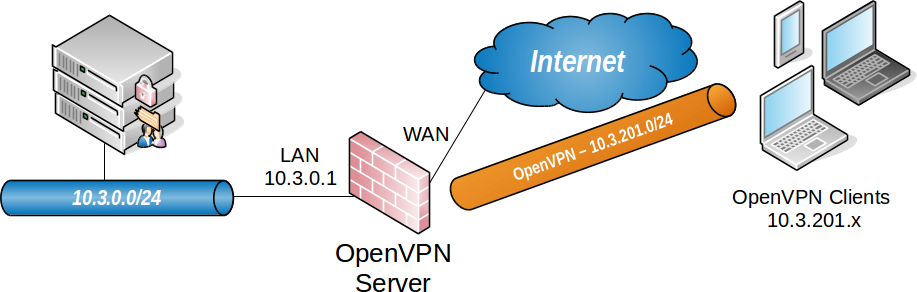
\includegraphics[width=0.99\linewidth]{images/openvpn-02.png} \end{center}

\begin{enumerate}
    \item dans \texttt{system/package manager/available packages}, installer: \textit{openvpn-client-export}
    \item sur \texttt{vpn/openvpn/wizards}, compléter le wizard:
    \begin{itemize}
        \item Description = VPN-R2S
        \item Tunnel Network = 10.0.4.0/24 (= réseau virtuel r2s)
        \item Local Network = 192.168.1.0/24, 10.0.0.0/24 (= réseaux lans)
        \item Firewall Rule = cocher la case
        \item OpenVPN Rule = cocher la case
    \end{itemize}
    \item sur \texttt{vpn/openvpn/client export utility}, aller en bas de la page, dans \textit{inline configurations}, cliquer sur \textit{most clients}
    \item exporter le fichier vers une machine debian:
    \begin{itemize}
        \item \texttt{sudo openvpn <fichier>.ovpn}
        \item \texttt{alt+f2}
        \item \texttt{ip route} (normalement, il y a les routes vers les lans du vpn)
        \item \texttt{ping 192.168.1.2} (= ip de la windows serveur dans le lan openvpn)
    \end{itemize}
\end{enumerate}
\textbf{Remarques}:
\begin{itemize}
    \item authentification via la db local [CR + mdp], il faut modifier les utilisateurs pour leur créer un certificat personnel (user manager)
    \item authentification radius [CR + mdp], il faut créer un certificat utilisateur normal (certificate manager)
\end{itemize}




















\newpage \tableofcontents




















\end{document}
